% =====================================================================================
% fig_rule_complexity.tex: how complex is each trunk unit as a rule, per layer (Q3;
%   companion of table_hoyer.tex; the depth limit of CLAUDE.md "rule-extraction limits").
%
% What the experiment tests: each conv unit is a threshold over binary literals; its
%   exact DNF is the set of its minimal covers. We measure, per unit, (a) the length of
%   its shortest rule (greedy minimum-cardinality bound, exact) and (b) the number of
%   its minimal covers (min_covers.count_min_covers; never enumerate a unit with ~1e10
%   covers), for the dense trunk and after layer-wise Hoyer, per layer L0 / L1 / L2.
% Plot: two panels. Left: shortest rule length per unit (box or violin per layer, dense
%   vs Hoyer side by side). Right: number of minimal covers per unit (log scale, same
%   layout). Dead units (no nonzero weight) shown as a separate count above each Hoyer box.
% What it shows: only L0 decodes to short rules (~3 literals); L1/L2 units need ~10-14
%   literals and have ~1e10 covers (weight diffusion, not a search limit); Hoyer brings L1
%   down to a few covers, partly by killing units.
% What it does not show: the explanation size of a prediction (that is set by the head
%   and the prototypes' cared bits, table_interp.tex); semantic quality of the rules.
% Data: final NMP (and NMP+QAT) checkpoints of E1, dense and after sparsify_proto.py;
%   min_covers.py on every unit.
% GENERATED BY: python plot_paper.py rule_complexity   (sources: configs/paper_figures.yaml, code:
%   utils/paper_figures.py, branch feat/paper-figures). "preliminary: true" in the config
%   stamps PRELIMINARY on the figure; set it to false only when every source is final.
% STATUS: PRELIMINARY version drawn 2026-10-21 (sum_ablation_ctrl NMP, 10 folds, dense vs low-lr layer-wise Hoyer). Final after E1 + the Hoyer post-hoc stage.
% TODO:
%   [ ] committed script computing per-unit bound + cover count (cheap, exact; guard
%       against enumeration) -> json per fold -> paper/figures/fig_rule_complexity.pdf.
%   [ ] appendix if table_hoyer goes to the appendix.
% =====================================================================================
\begin{figure}[t]
  \centering
  \IfFileExists{figures/fig_rule_complexity.pdf}{%
    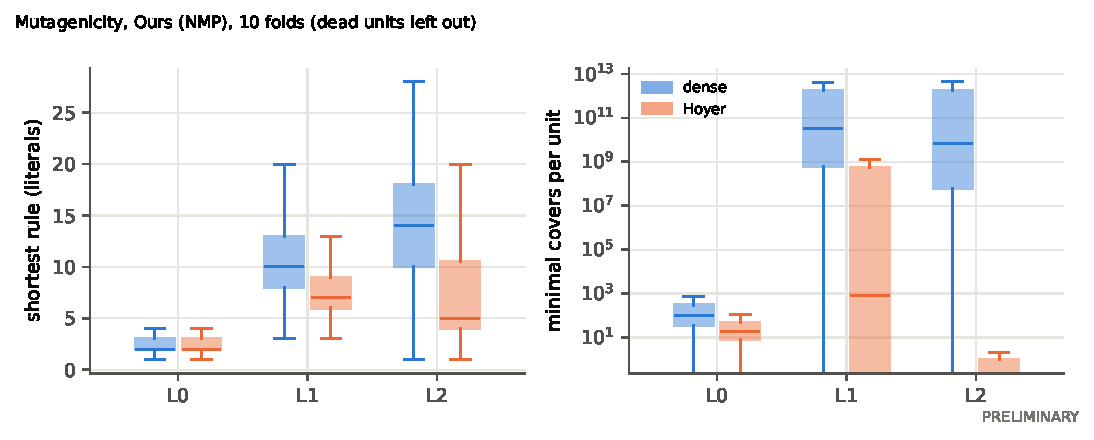
\includegraphics[width=\linewidth]{figures/fig_rule_complexity.pdf}%
  }{\fbox{\parbox[c][4cm]{0.95\linewidth}{\centering\todo{fig\_rule\_complexity.pdf: rule length and covers per layer}}}}
  \caption{Complexity of the trunk units as rules, per conv layer, for the dense trunk and
    after layer-wise Hoyer sparsification (Mutagenicity, \nmp{}, all folds). Left: length of
    the shortest rule. Right: number of minimal covers (DNF terms), log scale.}
  \label{fig:rule_complexity}
\end{figure}
